%-------------------------------------------------------------------------------
% File: main.tex
%       Formal Methods for Secure Systems project documentation.
%
%
% Author: Yuri Mazzuoli, Francesco Iemma
%         Created on 30/06/2021
%-------------------------------------------------------------------------------
\documentclass[11pt, a4paper, oneside]{book}

% equal left and right margins
\usepackage[hmarginratio=1:1]{geometry}

% configuration to typeset documents in english
\usepackage[english]{babel}

% include graphics in the file
\usepackage{graphicx}

% used in the dedication environment definition
\usepackage{afterpage}

% used to set page background image
\usepackage{tikz}

% used to handle math equations and formulas
\usepackage{amsmath}
\usepackage{mathtools}

% used to handle quotes
\usepackage{csquotes}

%used to handle bibliography
\usepackage{biblatex}

%used to change color and background color of single words
\usepackage{xcolor}

%used to place figures side by side
\usepackage{subfig}

%used to fix figure positioning
\usepackage{float}

%used to reference sections
\usepackage{hyperref}

\usepackage{mathtools}
\usepackage{amssymb}

% used to properly format table in appendix
\usepackage{multirow}

% used to rotate table in appendix
\usepackage{adjustbox}

% blank page command
\newcommand{\blankpage}
{
    \null
    \thispagestyle{empty}%
    \addtocounter{page}{-1}%
    \newpage
}

% dedication environment
\newenvironment{dedication}
{
    % blank page before dedication
    \afterpage{\blankpage}
    % we want a new page
    \clearpage
    % no header and footer
    \thispagestyle{empty}
    % some space at the top
    \vspace*{\stretch{1}}
    % the text is in italics
    \itshape
    % flush to the right margin
    \raggedleft
    % blank page after dedication
    \afterpage{\blankpage}
}
{
    % end the paragraph
    \par
    % space at bottom is one times that at the top
    \vspace{\stretch{1}}
    % finish off the page
    \clearpage
}

\newenvironment{specifications}
{
	\fontfamily{qtm}\selectfont
}{\par}

\usepackage[normalem]{ulem}
\useunder{\uline}{\ul}{}

%-------------------------------------------------------------------------------
% Title page
%-------------------------------------------------------------------------------
\title{
    \vspace{-3cm}
    
\includegraphics[scale=0.3]{img/cherubino_black.eps}\\
    {\scshape University of Pisa}\\
    School of Engineering\\
    \rule{7cm}{0.01cm}\\
    {\normalsize{\scshape Formal Methods for Secure Systems}}\\
    [2cm]
    {\scshape An ADVISE model for attacks on autonomous vehicles back-end servers}\\
    [3cm]
    \LARGE{\textbf{Supervisors}\hfill\textbf{Students}}\\
    \Large{\emph{Prof. Cinzia Bernardeschi}\hfill\emph{Yuri Mazzuoli\\}}
    \Large{\emph{Ing. Maurizio Palmieri}\hfill\emph{Francesco Iemma\\}}
    \Large{\hfill\emph{Marco Pinna\\}}
    \vfill
    \date{\today}
}

% leave the author field ampty in the title page
\author{}

%-------------------------------------------------------------------------------
% Document beginning
%-------------------------------------------------------------------------------
\begin{document}

% make title page
\maketitle

% enable page numbering back: roman numbers style
\pagenumbering{roman}

% print table of contents
\tableofcontents

% set arabic page numbering style
\pagenumbering{arabic}

%-------------------------------------------------------------------------------
% File: introduction.tex
%       Vehicle ADVISE project documentation.
%
% Author: Yuri Mazzuoli, Francesco Iemma, Marco Pinna
%         Created on 30/06/2021
%-------------------------------------------------------------------------------
\chapter{Introduction}\label{ch:introduction}
In this work the study of different adversaries trying to attack the back-end servers related to autonomous vehicles is carried out.\\

The work is organized as follows:
\begin{itemize}
    \item Firstly, chapter \ref{ch:overview} gives an initial overview and a presentation of the scenarios.
    \item Secondly, in chapter \ref{ch:attackTree} the complete attack tree is presented.
    \item In chapter \ref{ch:simulation} the development of the Mobius simulation is described and its results are presented.
\end{itemize}
    
\noindent
The entire codebase is available at \url{https://github.com/YuriMzz/vehiclesADVISE}.

% !TeX spellcheck = en_GB
%-------------------------------------------------------------------------------
% File: overview.tex
%       Vehicle ADVISE project documentation.
%
% Author: Yuri Mazzuoli, Francesco Iemma, Marco Pinna
%         Created on 30/06/2021
%-------------------------------------------------------------------------------
\chapter{Overview}\label{ch:overview}

In this chapter a general overview of the scenarios and the involved actors is given.

\section{Actors} %TODO change to adversaries?
\noindent In our model we have three different types of actors:
\begin{itemize}
	\item Hacker
	
	\noindent (S)he is a malicious person with an in-depth knowledge of the most important and widespread technologies and attacks. For this reasons he is the most skilled user.
	
	\item Insider
	
	\noindent (S)he is a person who is inside the organization and so he has more accesses w.r.t. an outsider attacker and in particular he has a lot of knowledges, on the other side he has not the same skill level of the hacker.
	
	\item Physical Intruder
	
	\noindent (S)he is a person who is able to have physical access to the infrastructures under analysis. The physical intruder can be an insider with particular privileges (e.g. access to the server room) or also an hacker who was able to retrieve in a malicious way the physical access to the infrastructures.
\end{itemize}


\noindent TODO: mettere una tabella con le skill, le conoscenze e gli accessi a disposizione di ogni attaccante
%-------------------------------------------------------------------------------
% File: attackTree.tex
%       Vehicle ADVISE project documentation.
%
% Author: Yuri Mazzuoli, Francesco Iemma, Marco Pinna
%         Created on 30/06/2021
%-------------------------------------------------------------------------------
\chapter{Attack tree}\label{ch:attackTree}


\begin{figure}[H]
    \begin{center}
        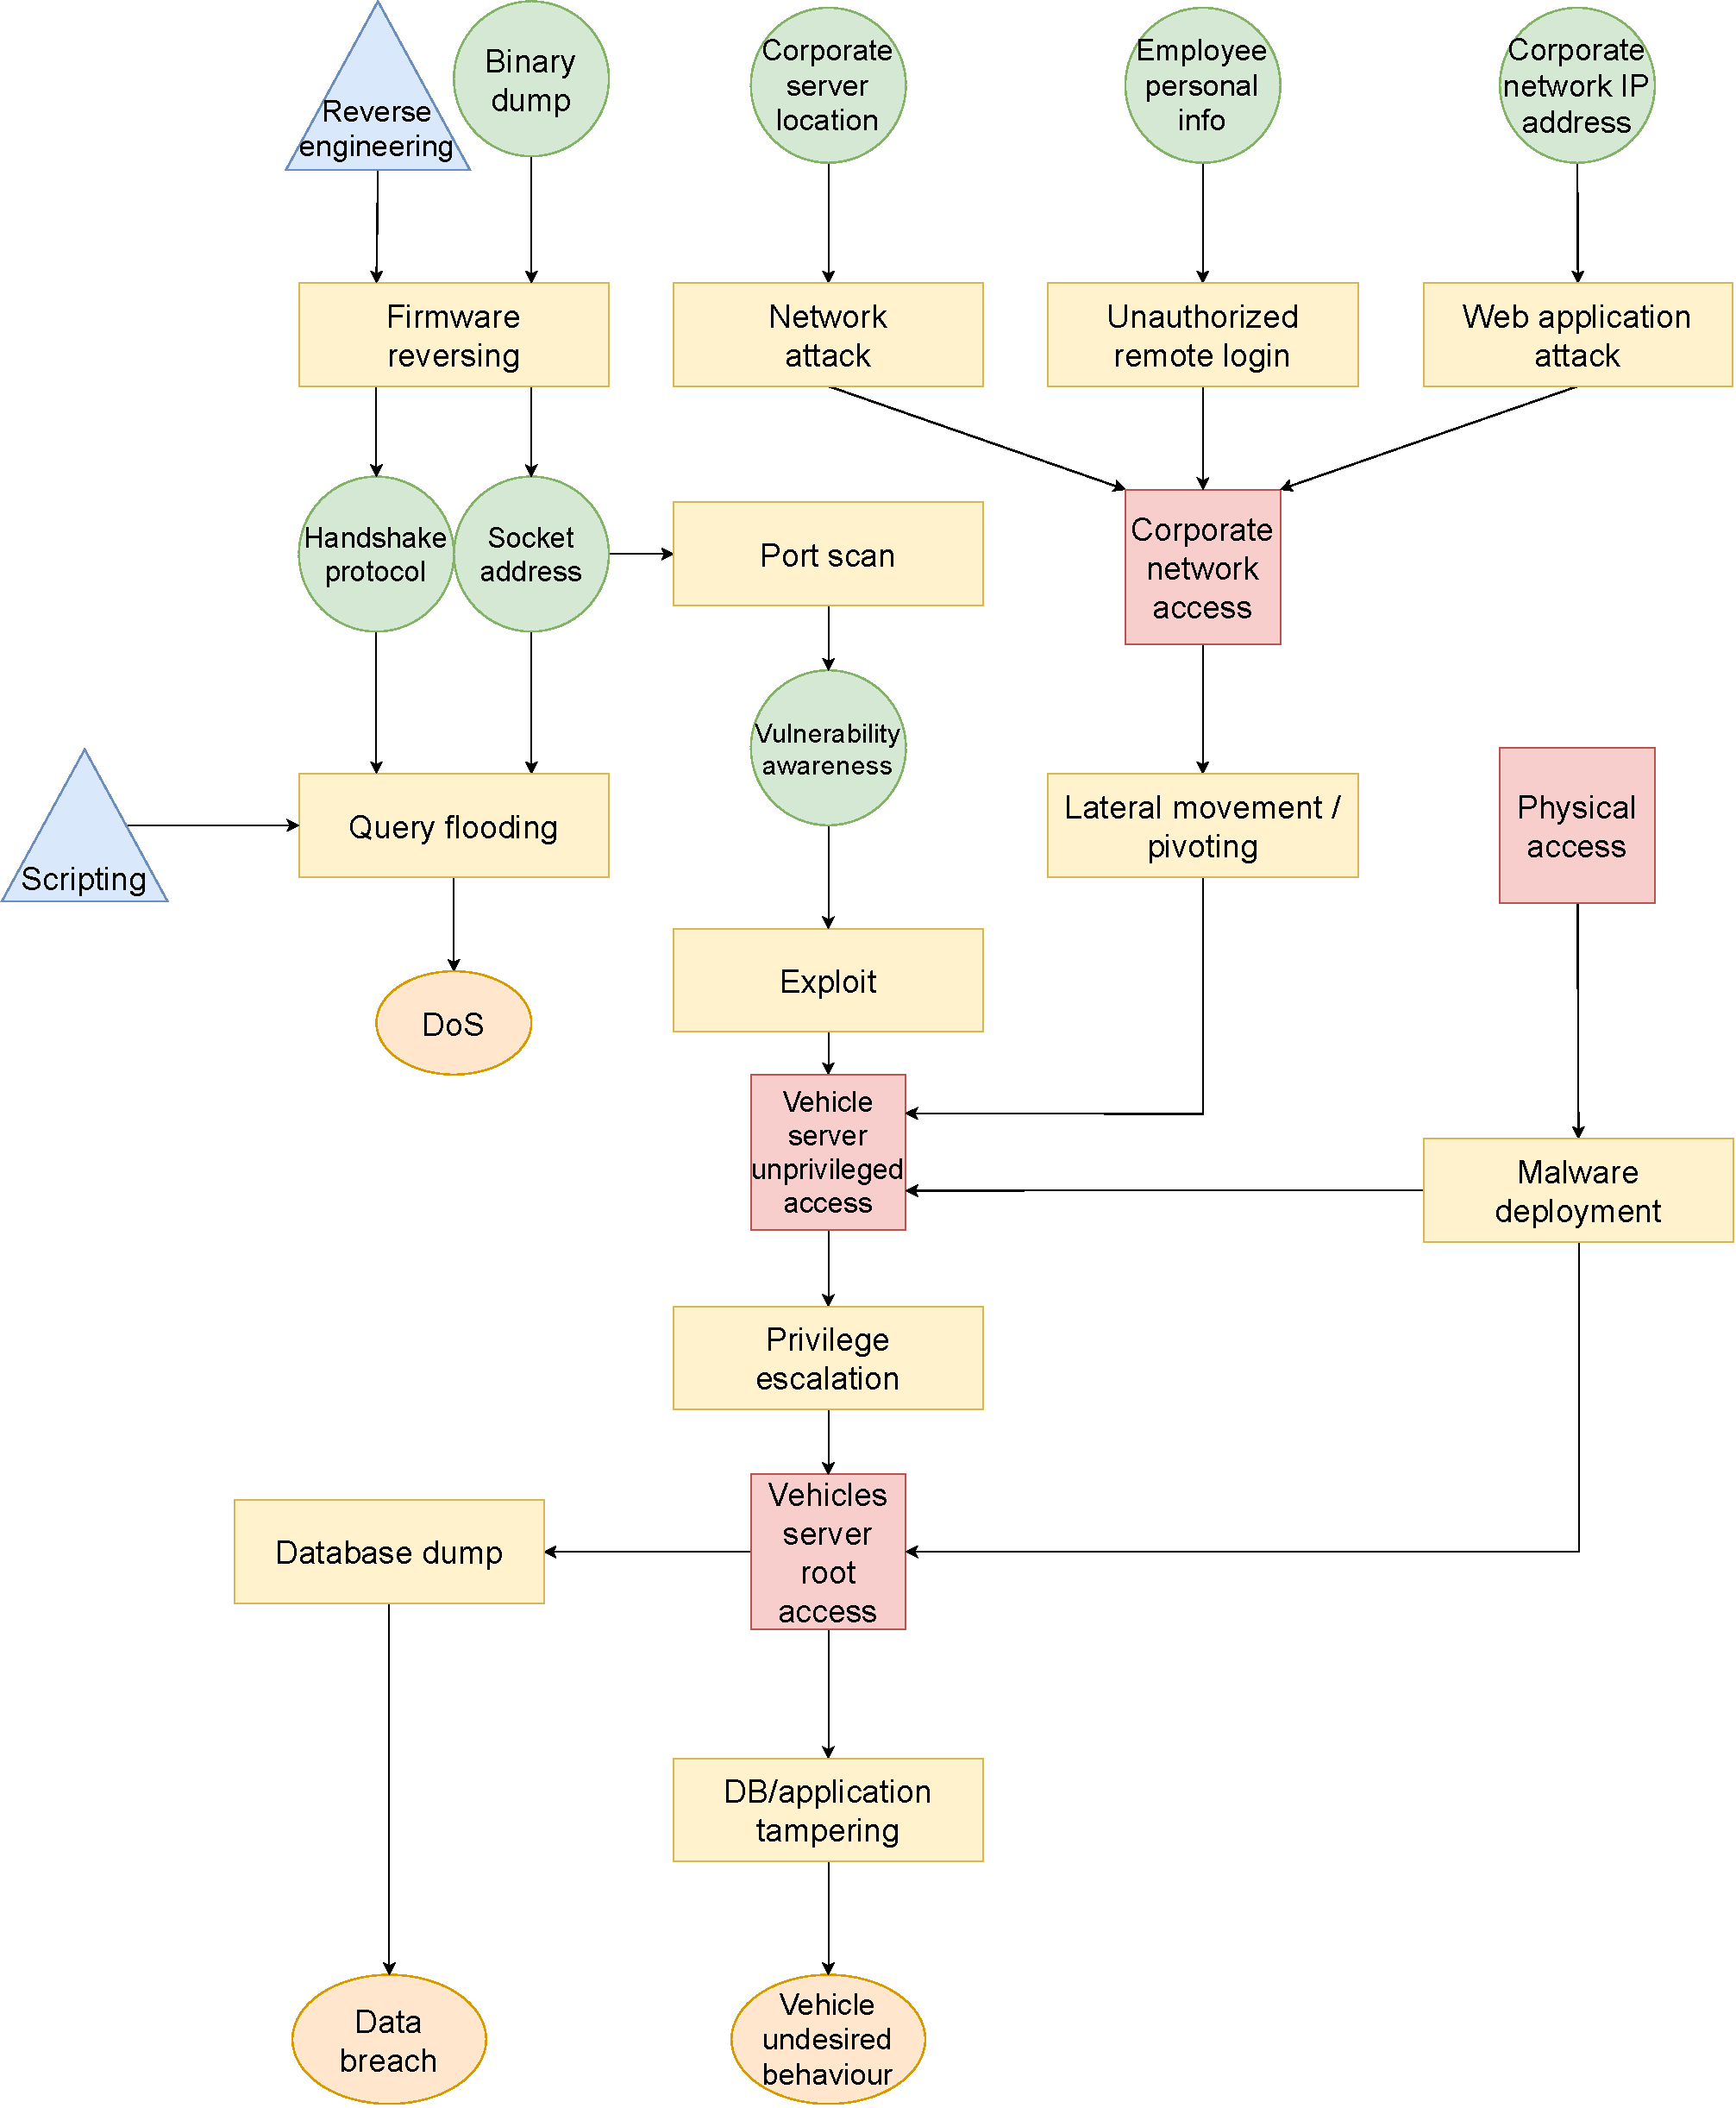
\includegraphics[scale=0.3]{img/attackTree.pdf}
        \caption{Attack tree}
        \label{fig:attackTree}
    \end{center}
    \vspace*{-0.4cm}
\end{figure}
% !TeX spellcheck = en_GB
%-------------------------------------------------------------------------------
% File: simulation.tex
%       Vehicle ADVISE project documentation.
%
% Author: Yuri Mazzuoli, Francesco Iemma, Marco Pinna
%         Created on 30/06/2021
%-------------------------------------------------------------------------------
\chapter{Simulation}\label{ch:simulation}

We implemented the attack tree in Mobius Tool in order to get some insights about the
attackers behaviour and the most dangerous attack paths. 
We took an heuristic approach in order to evaluate cost and duration of different attacks; the time unit for attacks is \textit{hours}.
\section{General Results}
We decided to simulate 200 units of time (200 h) with Mobius in order to evaluate each attacker's results for 
different configuration of mitigations. The following general results were obtained:\\
\begin{itemize}
    \item the \textbf{Hacker} will always try to achieve the most remunerative goals, despite the
        possibility to be detected; 
    \item the \textbf{Physical intruder} will try to achieve only the most remunerative goal, and will
        ignore the others because of the high probability of being detected (reward-risk ratio is too low)
    \item the \textbf{Insider} has the same behaviour as the Physical intruder, but for them the probability
        to reach the goal increases faster because their attack path has a higher success probability.
\end{itemize}
\newpage
\section{Hacker Attacks}
\subsection*{DoS}
When no mitigations are applied, the Hacker will rarely try to obtain a DoS, but they will commit themselves
to other attacks in order to obtain high reward goals. Introducing \textbf{CodeObfuscation}, binary reversing
become harder to complete with success, leading to a probability of reaching the DoS goal near to 0.\\
Increasing the firewall sensitivity will indeed increase the probability for the hacker to reach the DoS,
because they will give up on trying to reach other goals, focusing only on this one.
\begin{figure}[H]
    \begin{center}
        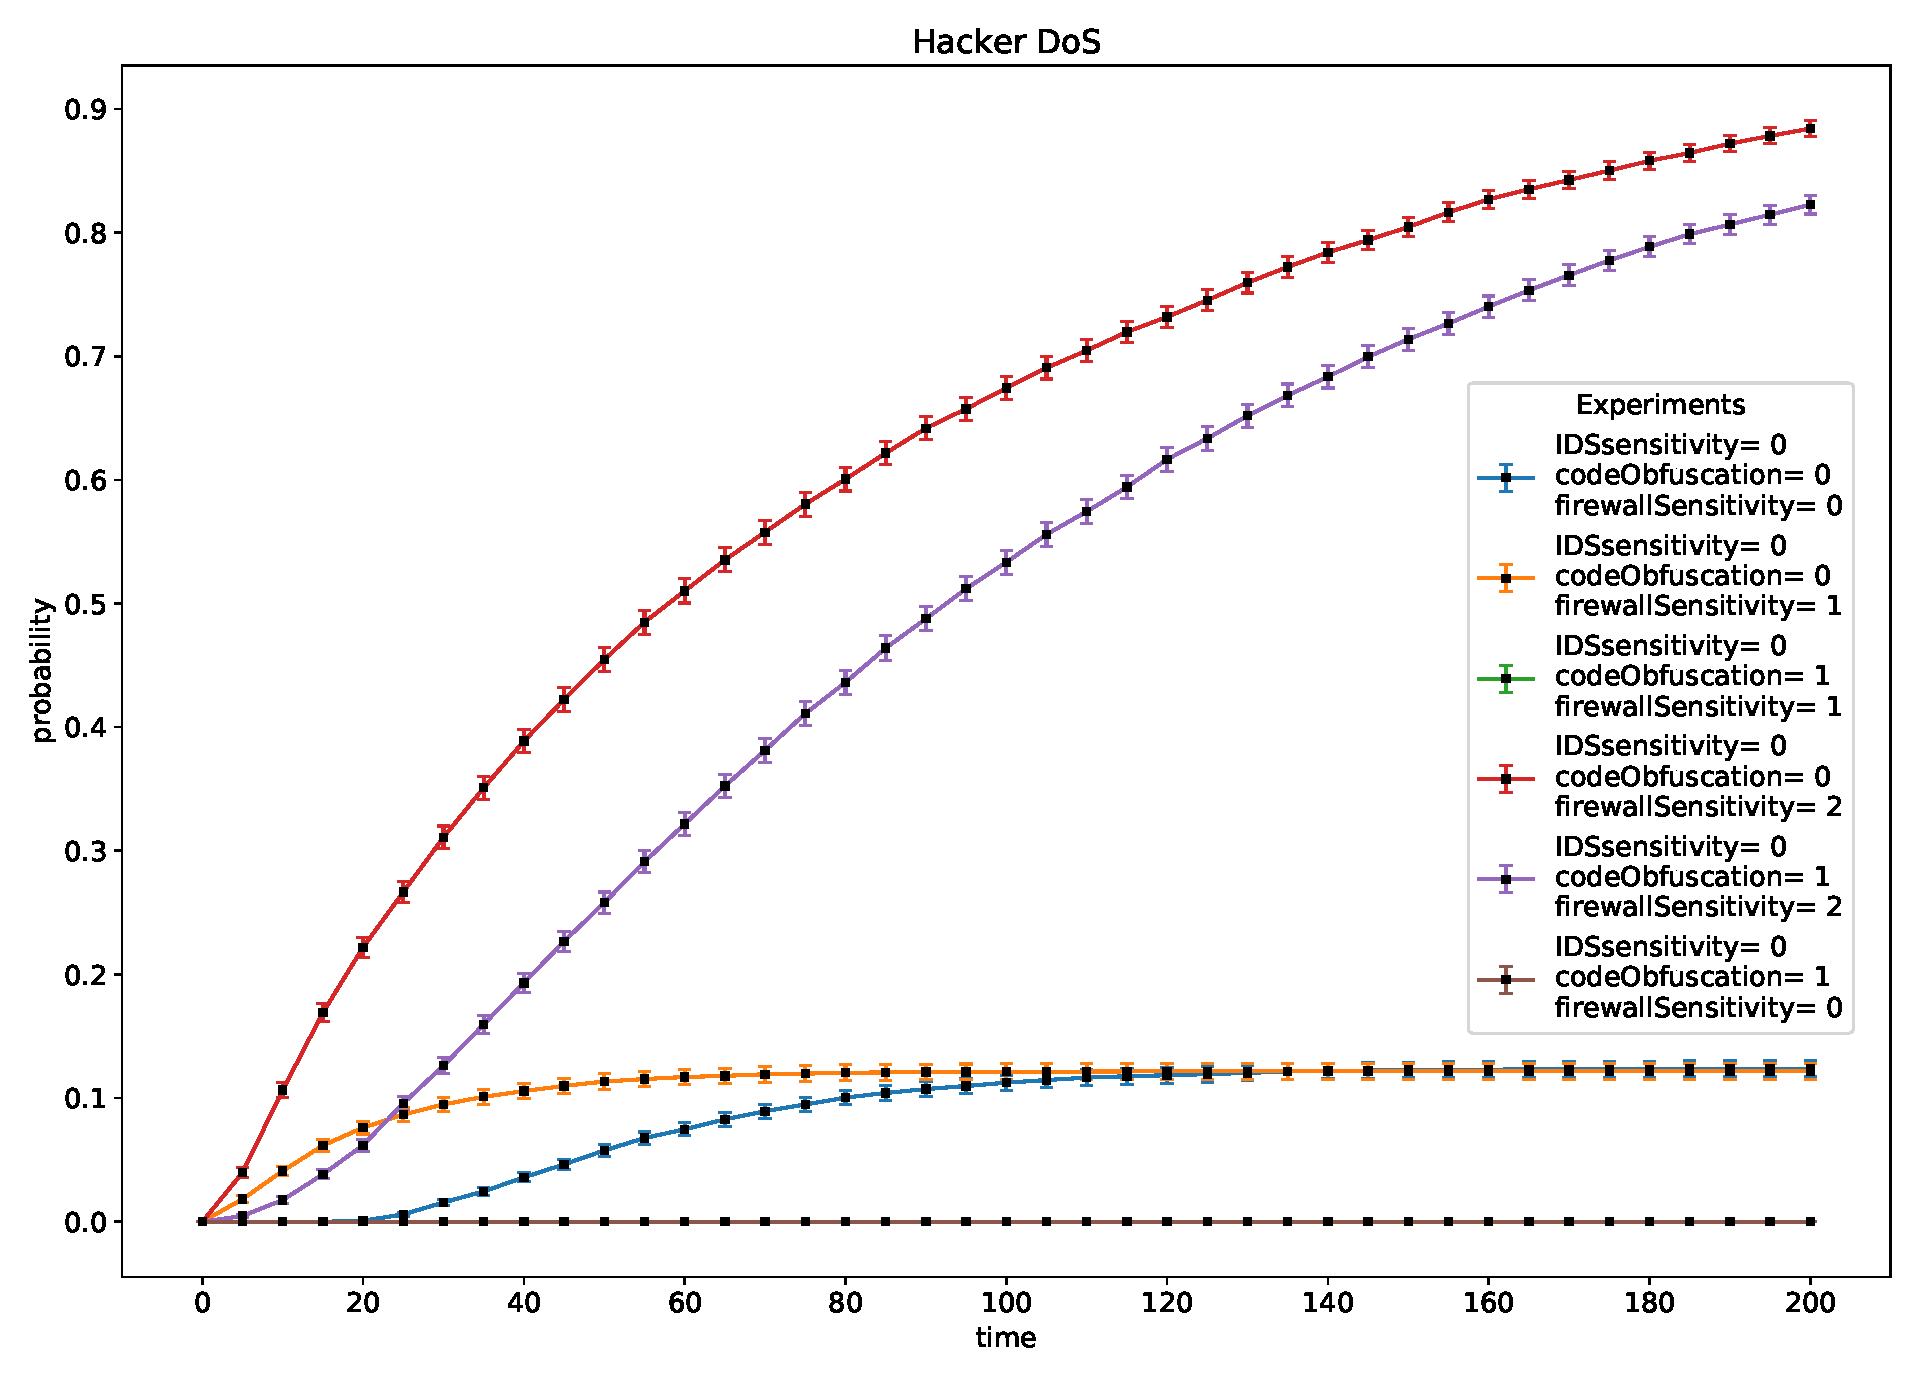
\includegraphics[scale=0.45]{img/Hacker_DoS.pdf}
    \end{center}
    \caption{Hacker DoS}
    \label{fig:Hacker_DoS}
    \vspace*{-0.8cm}
\end{figure}
\newpage
\subsection*{Data Breach and Vehicle Undesidered Behaviour}
When no mitigations are applied, the Hacker will reach these goals pretty fast. Introducing \textbf{CodeObfuscation}
will slow them down, but increasing \textbf{Firewall Sensitivity} we are able to reduce their will to reach them
until they will give up. 
\begin{figure}[H]
    \begin{center}
        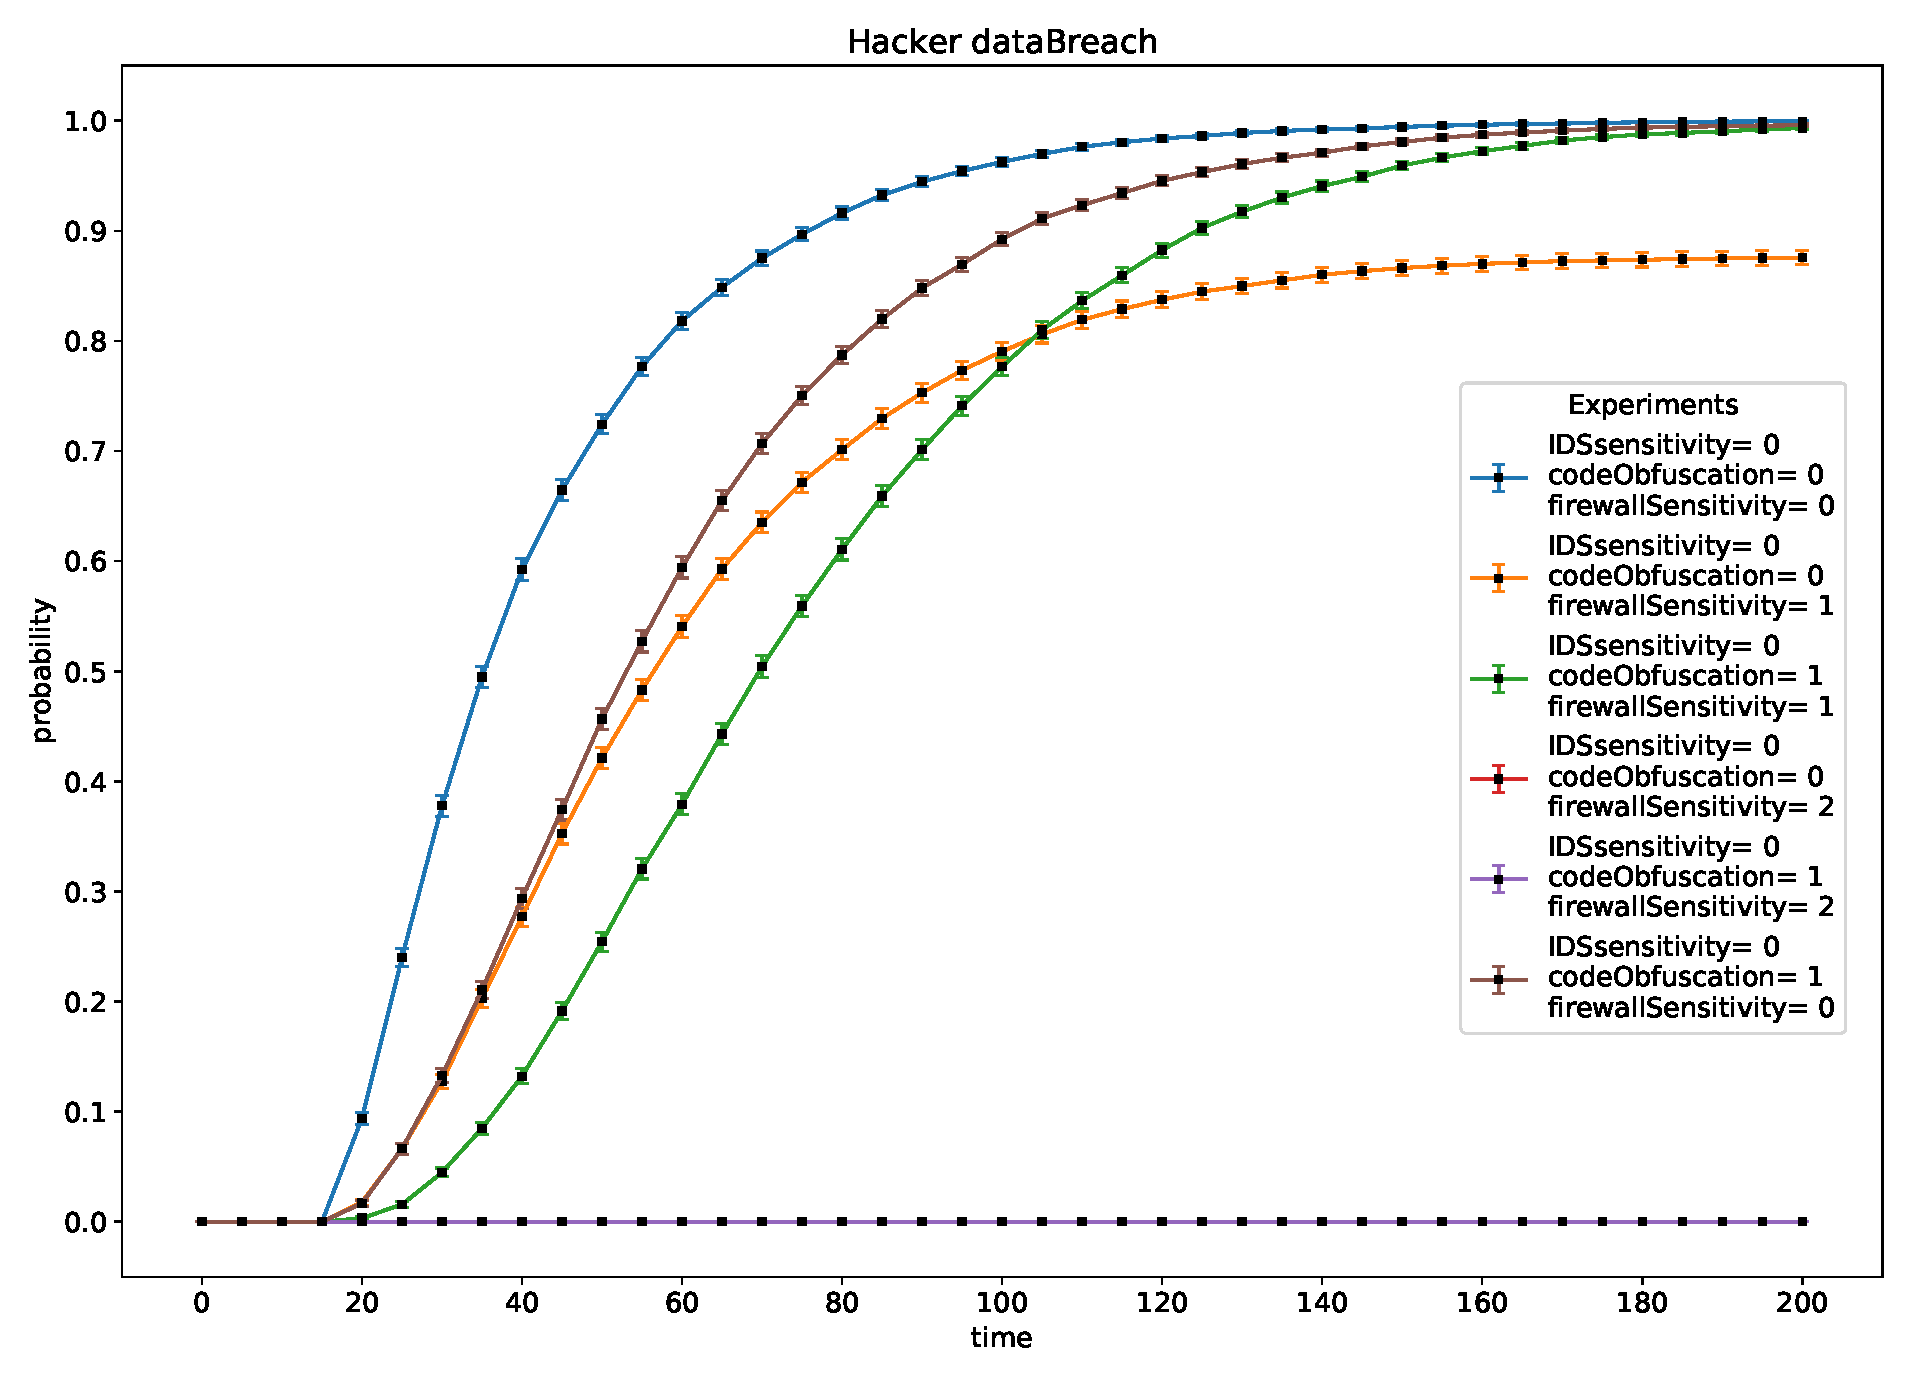
\includegraphics[scale=0.4]{img/Hacker_dataBreach.pdf}
        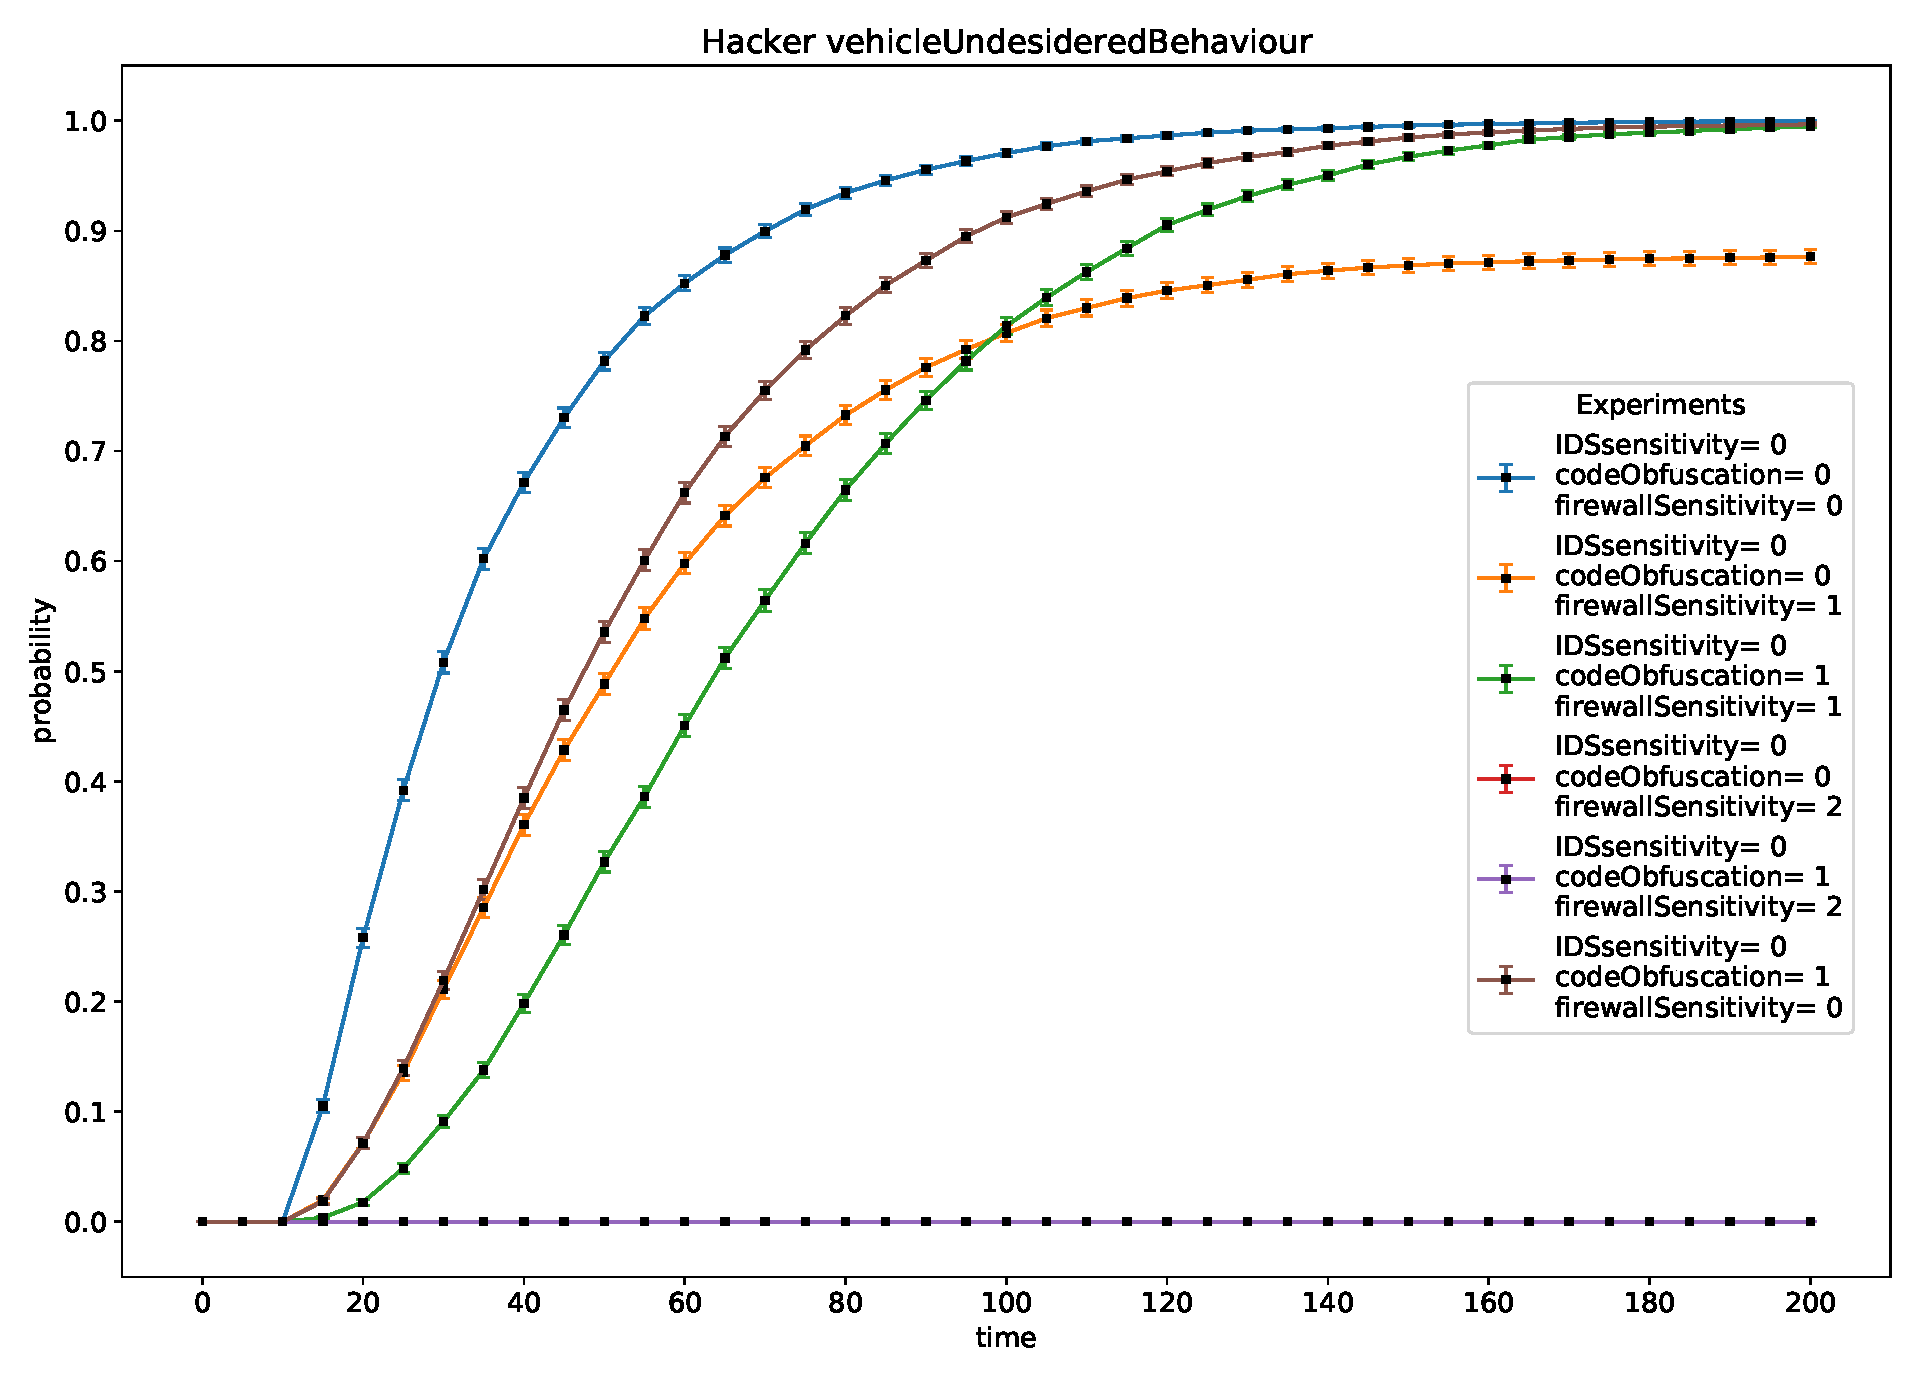
\includegraphics[scale=0.4]{img/Hacker_vOB.pdf}
    \end{center}
    \caption{Hacker Data Breach and Vehicle Undesidered Behaviour}
    \label{fig:Hacker_dataBreach}
    \vspace*{-2cm}
\end{figure}
\section{Physical Intruder and Insider Attacks}

\subsection*{Vehicle Undesired Behaviour}
When no mitigations are applied, both attackers will reach this goal pretty fast. Increasing 
\textbf{Intrusion Detection System Sensitivity}, we are able to reduce their will to reach the goal
until they will give up, because the probability to be discovered will be to high.
\begin{figure}[H]
    \begin{center}
        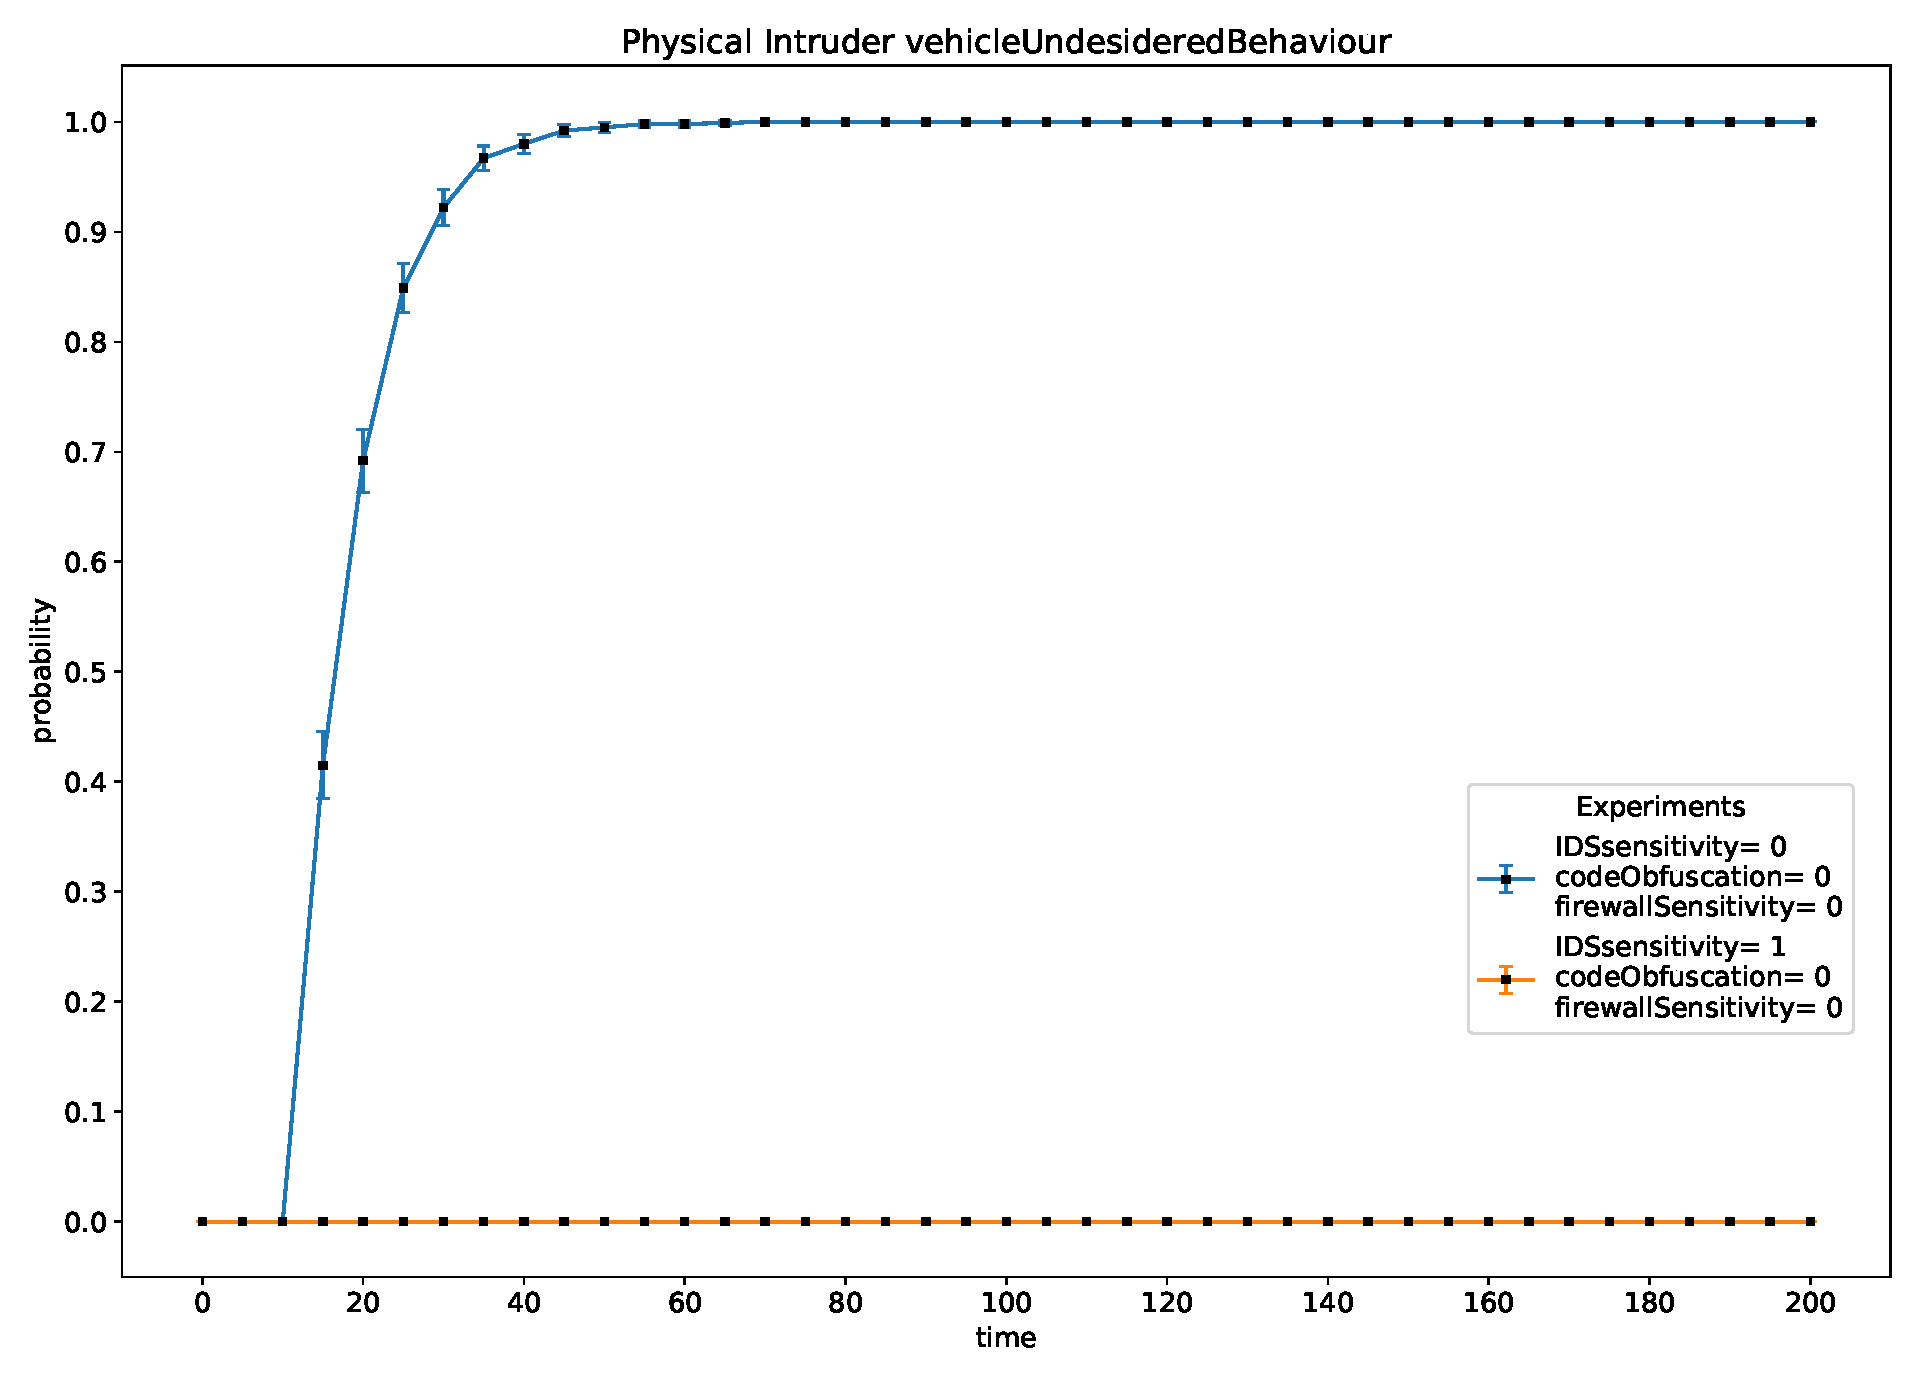
\includegraphics[scale=0.38]{img/Physical_vOB.pdf}
        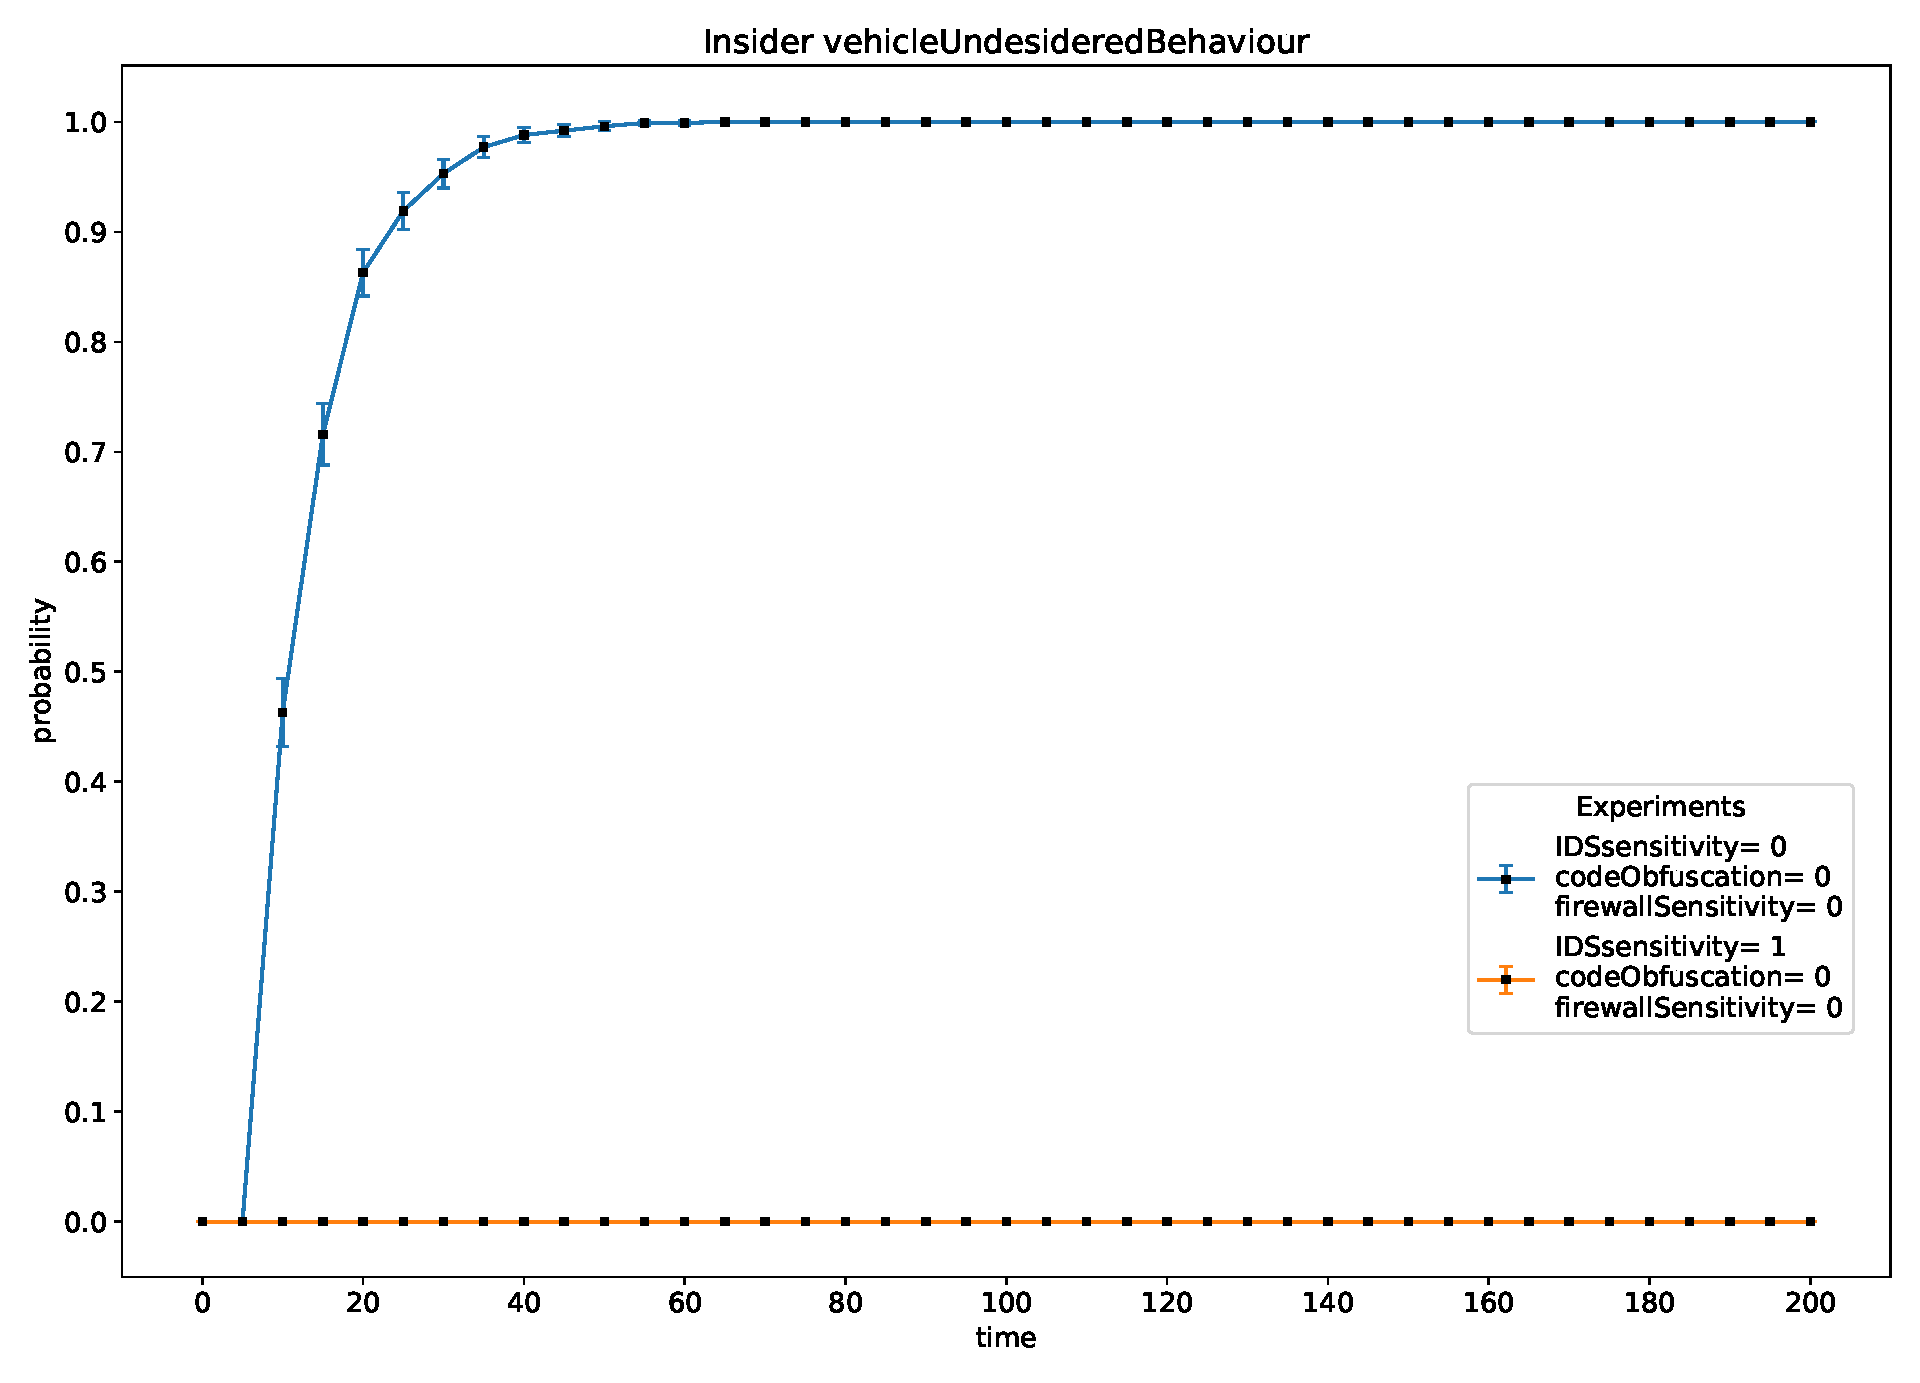
\includegraphics[scale=0.38]{img/Insider_vOB.pdf}
    \end{center}
    \caption{Physical intruder and Insider Vehicle Undesidered Behaviour}
    \label{fig:P_I_vob}
    \vspace*{-3cm}
\end{figure}

It is important to underline that in the case of an insider attacker, the time needed to achieve a high probability is lower w.r.t. the one needed for a physical intruder, since the two attackers follow different paths and the one taken by the physical intruder is longer and requires more time.

\section{Conclusion}
\noindent At the end of our analysis we can infer that is a very good idea to invest in a highly reliable and effective \textbf{Firewall} in order to discourage attacks from the hacker; furthermore IDS and code obfuscation techniques proved to be good countermeasures too.
Therefore implementing these mitigations results in an improvement in the overall security of the system.

% !TeX spellcheck = en_GB
%-------------------------------------------------------------------------------
% File: appendix.tex
%       Vehicle ADVISE project documentation.
%
% Author: Yuri Mazzuoli, Francesco Iemma, Marco Pinna
%         Created on 30/06/2021
%-------------------------------------------------------------------------------
\chapter{Appendices}\label{ch:appendices}
\section*{Appendix A}
\begin{table}[h]
\centering
\resizebox{\textwidth}{!}{\begin{tabular}{|l|l|l|l|l|}
\hline
\multicolumn{3}{|c|}{\textit{High level and sub-level descriptions of vulnerability/ threat}}                                                                                                                                                                                                                        & \multicolumn{2}{c|}{\textit{Example of vulnerability or attack method}}                                                                                                                                  \\ \hline
\multirow{9}{*}{\begin{tabular}[c]{@{}l@{}}4.3.1 Threats\\ regarding back-end\\ servers related to\\ vehicles in the field\end{tabular}} & \multirow{3}{*}{1} & \multirow{3}{*}{\begin{tabular}[c]{@{}l@{}}Back-end servers used as a\\ means to attack a vehicle or\\ extract data\end{tabular}}                    & 1.1 & Abuse of privileges by staff (\textbf{insider attack})                                                                                                                                                      \\ \cline{4-5} 
                                                                                                                                         &                    &                                                                                                                                                      & 1.2 & \begin{tabular}[c]{@{}l@{}}\textbf{Unauthorized internet access} to the server (enabled\\ for example by backdoors, unpatched system\\ software vulnerabilities, SQL attacks or other means)\end{tabular}   \\ \cline{4-5} 
                                                                                                                                         &                    &                                                                                                                                                      & 1.3 & \begin{tabular}[c]{@{}l@{}}\textbf{Unauthorized physical access} to the server\\ (conducted by for example USB sticks or other\\ media connecting to the server)\end{tabular}                               \\ \cline{2-5} 
                                                                                                                                         & 2                  & \begin{tabular}[c]{@{}l@{}}Services from back-end server\\ being disrupted, affecting the\\ operation of a vehicle\end{tabular}                      & 2.1 & \begin{tabular}[c]{@{}l@{}}\textbf{Attack on back-end server stops it functioning},\\ for example it prevents it from interacting with\\ vehicles and providing services they rely on\end{tabular}          \\ \cline{2-5} 
                                                                                                                                         & \multirow{5}{*}{3} & \multirow{5}{*}{\begin{tabular}[c]{@{}l@{}}Vehicle related data held on\\ back-end servers being lost or\\ compromised ("data breach")\end{tabular}} & 3.1 & Abuse of privileges by staff (\textbf{insider attack})                                                                                                                                                      \\ \cline{4-5} 
                                                                                                                                         &                    &                                                                                                                                                      & 3.2 & \begin{tabular}[c]{@{}l@{}}\textbf{Loss of information in the cloud}. Sensitive data\\ may be lost due to attacks or accidents when data is\\ stored by third-party cloud service providers\end{tabular}    \\ \cline{4-5} 
                                                                                                                                         &                    &                                                                                                                                                      & 3.3 & \begin{tabular}[c]{@{}l@{}}\textbf{Unauthorized internet access to the server}\\ (enabled for example by backdoors, unpatched\\ system software vulnerabilities, SQL attacks or other\\ means)\end{tabular} \\ \cline{4-5} 
                                                                                                                                         &                    &                                                                                                                                                      & 3.4 & \begin{tabular}[c]{@{}l@{}}\textbf{Unauthorized physical access to the server}\\ (conducted for example by USB sticks or other\\ media connecting to the server)\end{tabular}                               \\ \cline{4-5} 
                                                                                                                                         &                    &                                                                                                                                                      & 3.5 & \begin{tabular}[c]{@{}l@{}}\textbf{Information breach} by unintended sharing of data\\ (e.g. admin errors)\end{tabular}                                                                                     \\ \hline
\end{tabular}}
\end{table}




\end{document}
